\begin{frame}
\frametitle{Real data}
\begin{columns}[c]
\column{0.5\textwidth}
Used 550 T1w brain MRI from IXI ({\bf I}nformation e{\bf X}traction from {\bf I}mages) dataset.\par
\url{http://www.brain-development.org/}\par
Data from three different hospitals in London:
\begin{itemize}
\item{Hammersmith Hospital using a Philips 3T system}
\item{Guy's Hospital using a Philips 1.5T system}
\item{Institute of Psychiatry using a GE 1.5T system}
\end{itemize}

\column{0.5\textwidth}
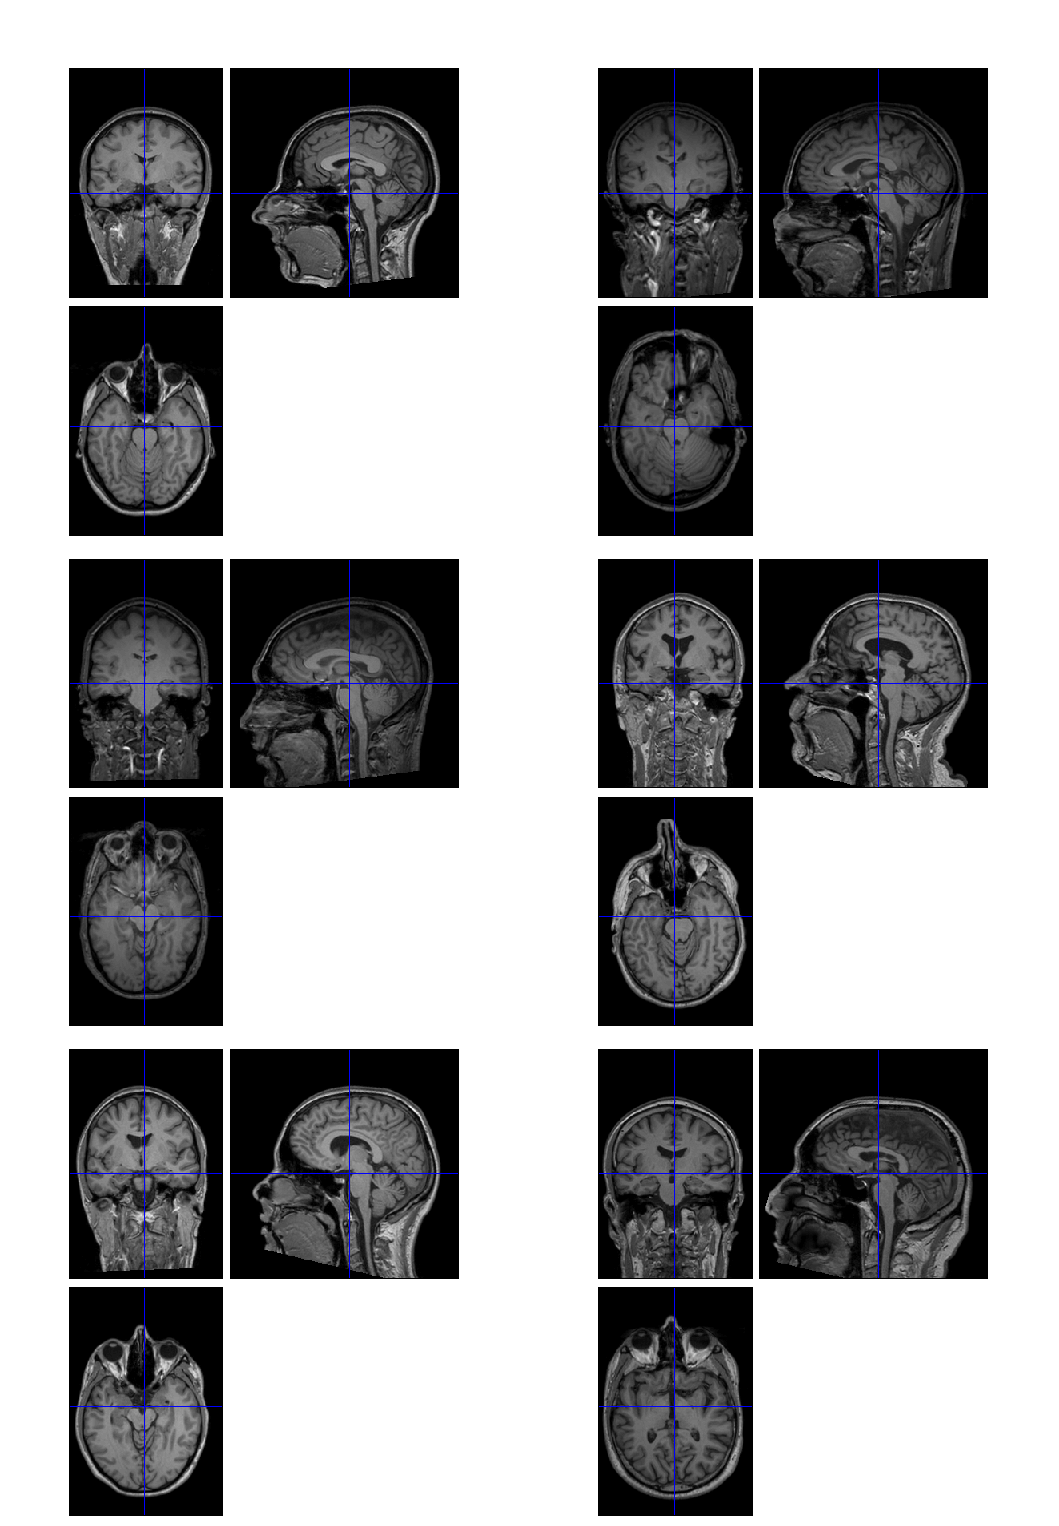
\includegraphics[width=0.9\textwidth]{orig_ixi}
\end{columns}
\end{frame}



\begin{frame}
\frametitle{Grey and White Matter}
\begin{columns}[c]
\column{0.26\textwidth}
Segmented into GM and WM.

Approximately aligned via rigid-body.
\column{0.75\textwidth}
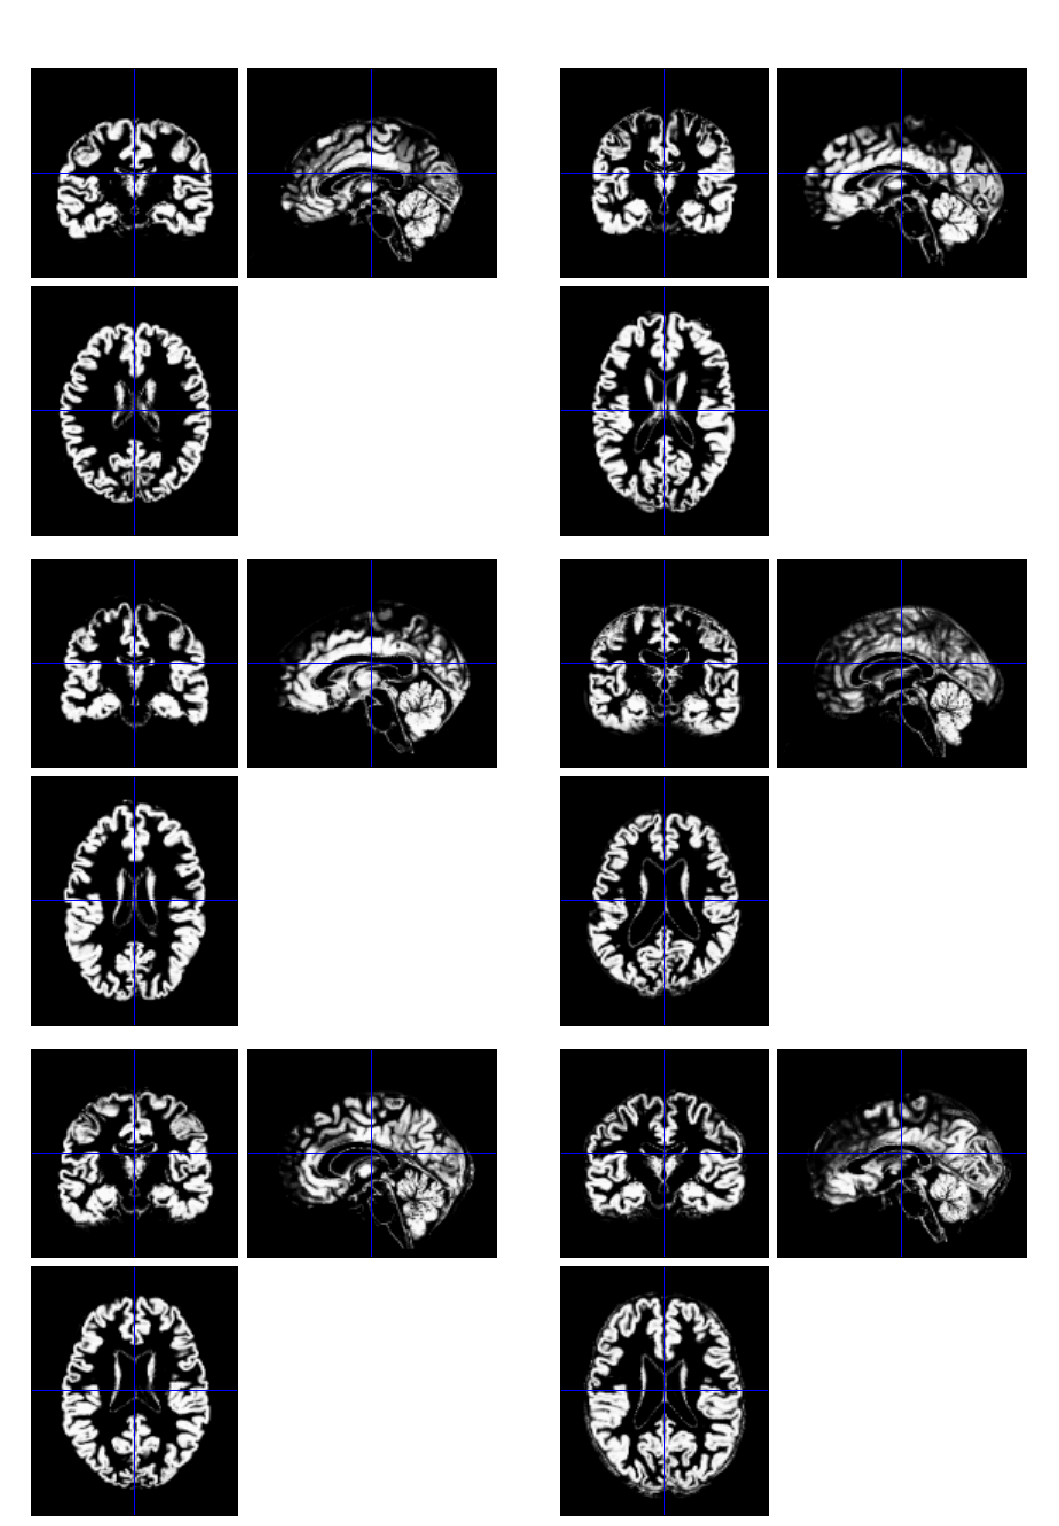
\includegraphics[width=0.5\textwidth]{gm_ixi}
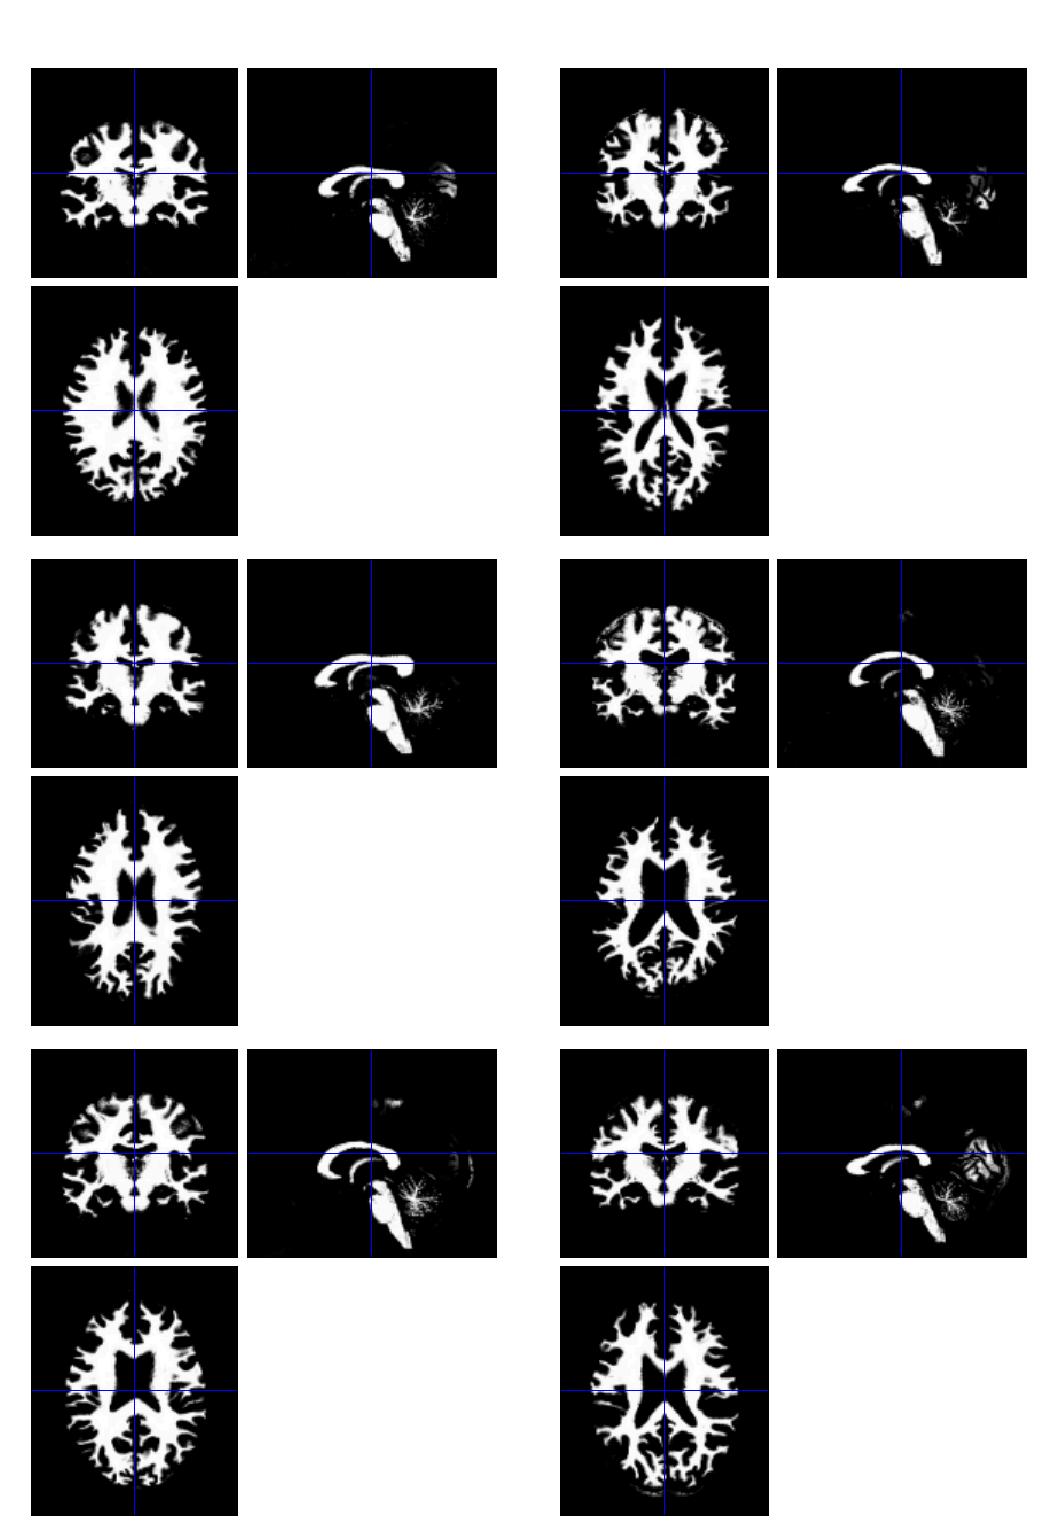
\includegraphics[width=0.5\textwidth]{wm_ixi}
\end{columns}

\begin{tiny}
Ashburner, J \& Friston, KJ. \emph{Unified segmentation}. NeuroImage 26(3):839--851 (2005).\par
\end{tiny}
\end{frame}



\begin{frame}
\frametitle{Diffeomorphic Alignment}
All GM and WM were diffeomorphically aligned to their common average-shaped template.
\begin{center}
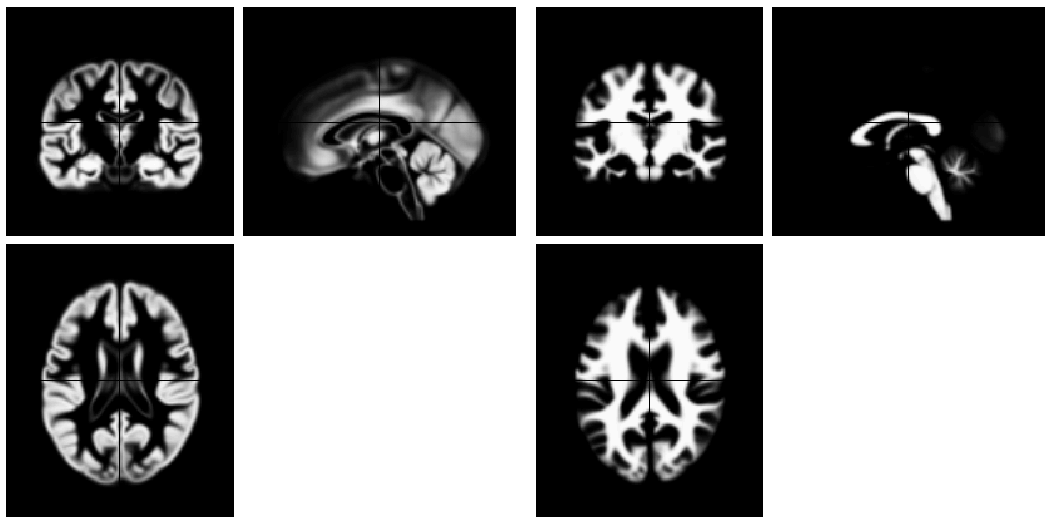
\includegraphics[width=.8\textwidth]{template}
\end{center}

\begin{tiny}
Ashburner, J \& Friston, KJ. \emph{Diffeomorphic registration using geodesic shooting and Gauss-Newton optimisation}. NeuroImage 55(3):954--967 (2011).\par
Ashburner, J \& Friston, KJ. \emph{Computing average shaped tissue probability templates}. NeuroImage 45(2):333--341 (2009).\par
\end{tiny}
\end{frame}



\begin{frame}
\frametitle{Volumetric Features}
\begin{columns}[c]
\column{0.33\textwidth}
A number of features were used for pattern recognition.

Firstly, two features relating to relative volumes.

Initial velocity divergence is similar to logarithms of Jacobian determinants.
\column{0.33\textwidth}
Jacobian Determinants

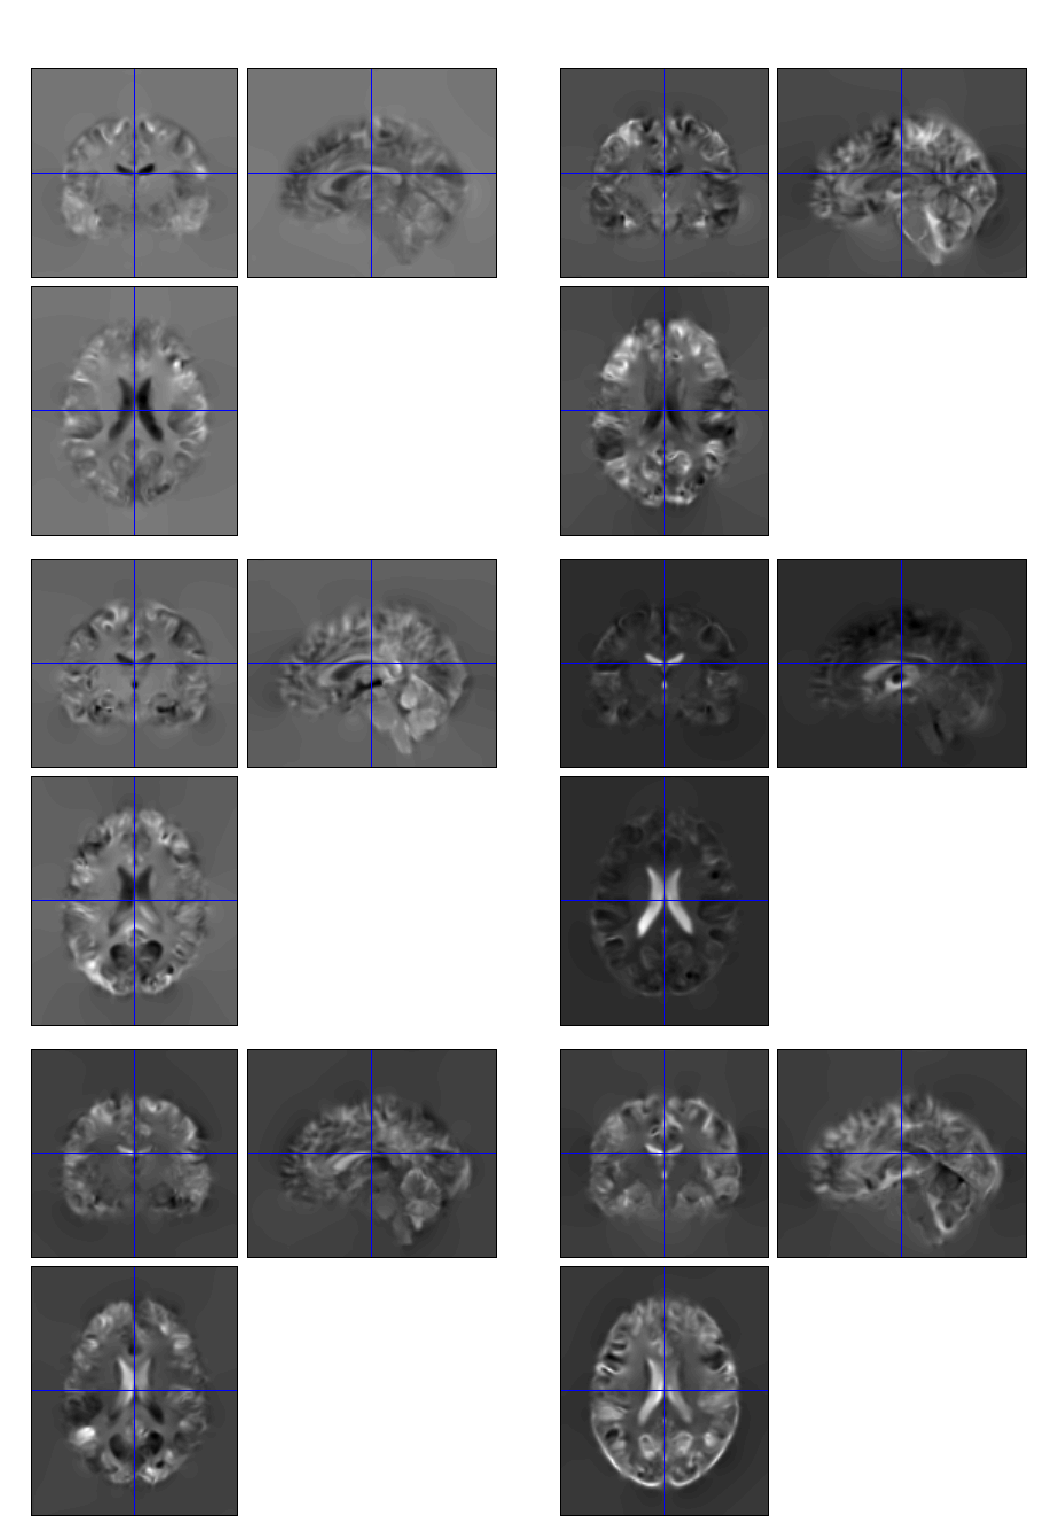
\includegraphics[width=1\textwidth]{jac_ixi}
\column{0.33\textwidth}
Initial Velocity Divergence
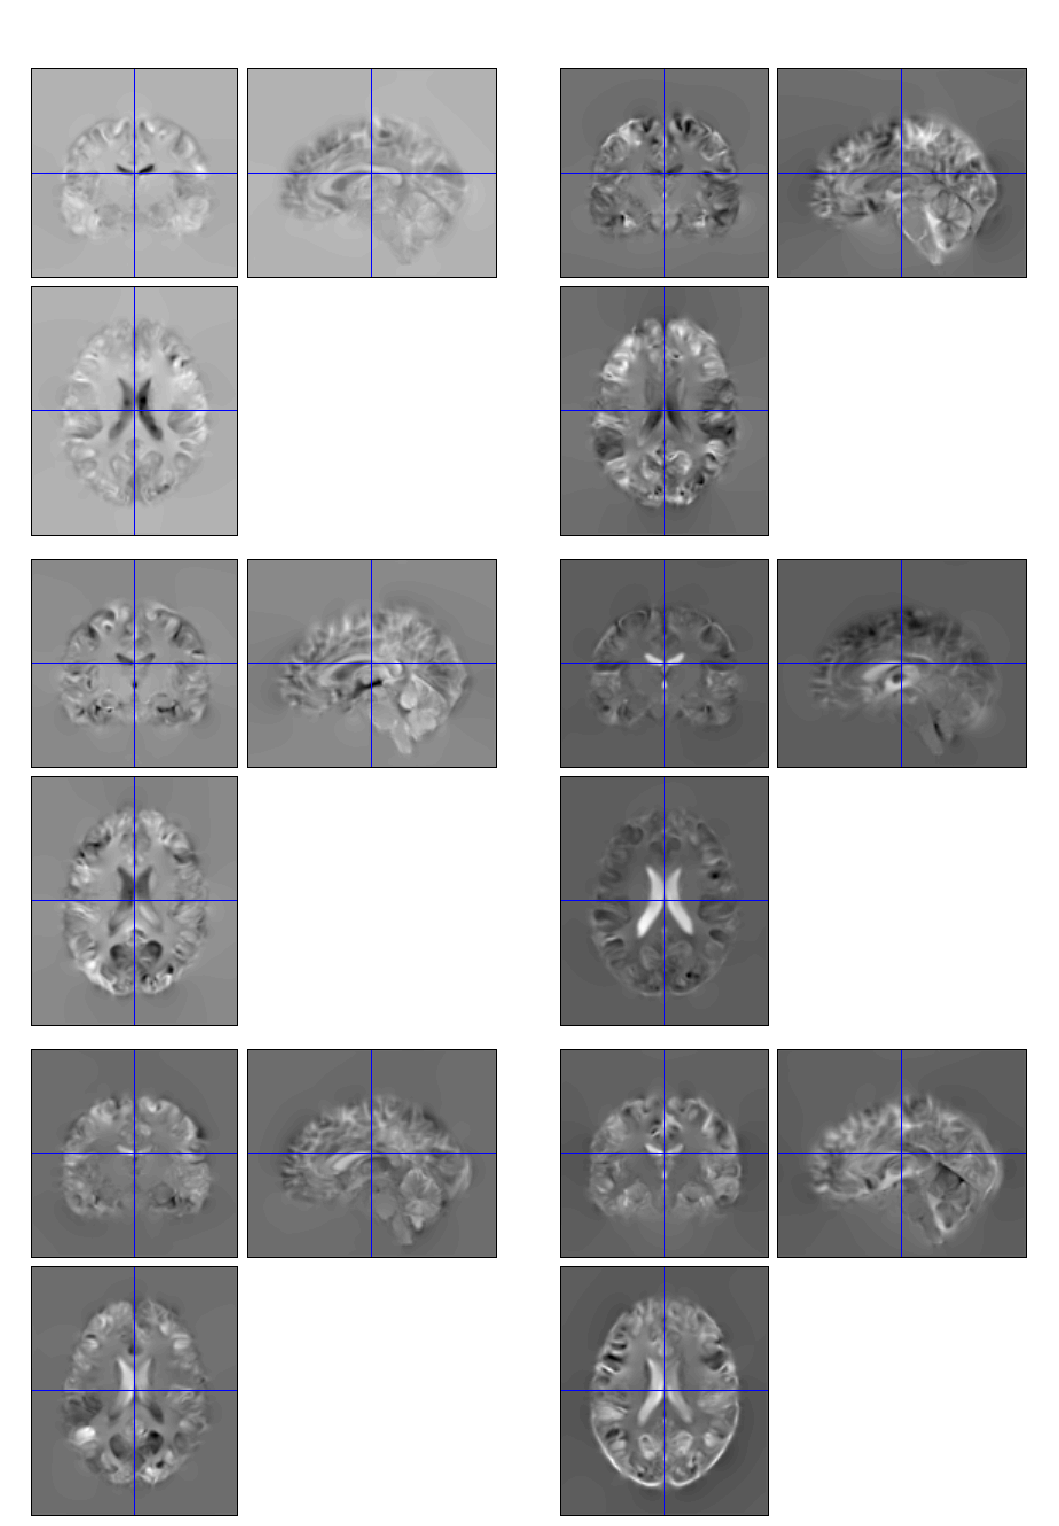
\includegraphics[width=1\textwidth]{div_ixi}
\end{columns}
\end{frame}



\begin{frame}
\frametitle{Grey Matter Features}
\begin{columns}[c]
\column{0.33\textwidth}
Rigidly Registered GM

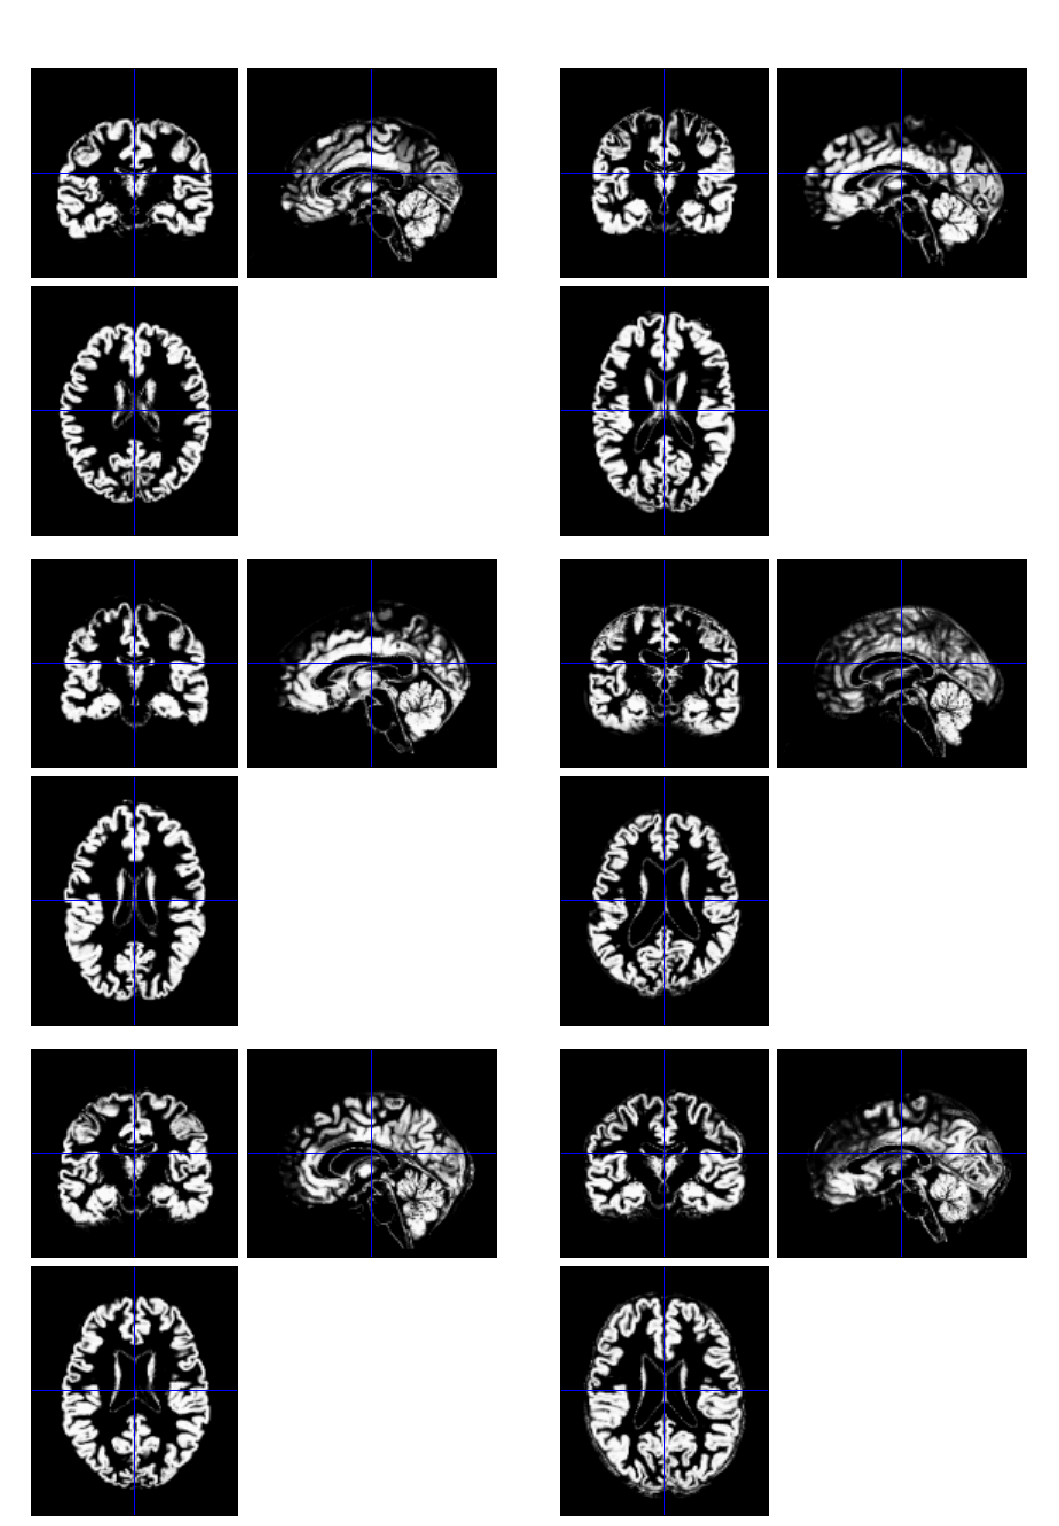
\includegraphics[width=1\textwidth]{gm_ixi}

\column{0.33\textwidth}
Nonlinearly Registered GM

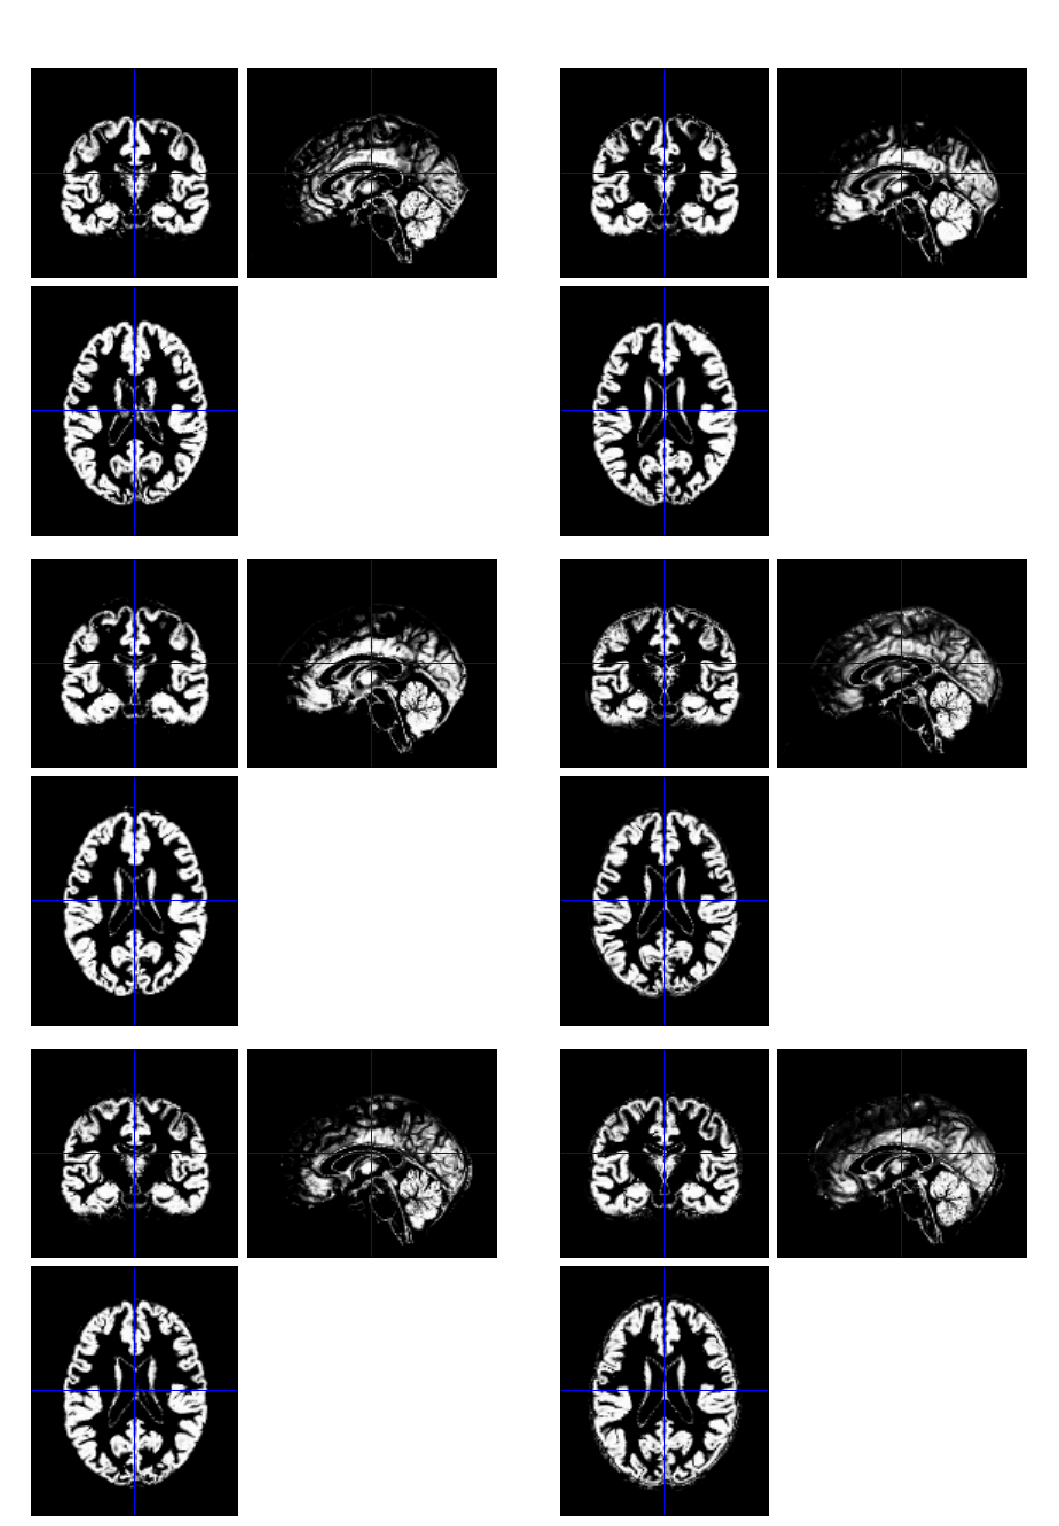
\includegraphics[width=1\textwidth]{wc1_ixi}
\column{0.33\textwidth}
Registered and Jacobian Scaled GM

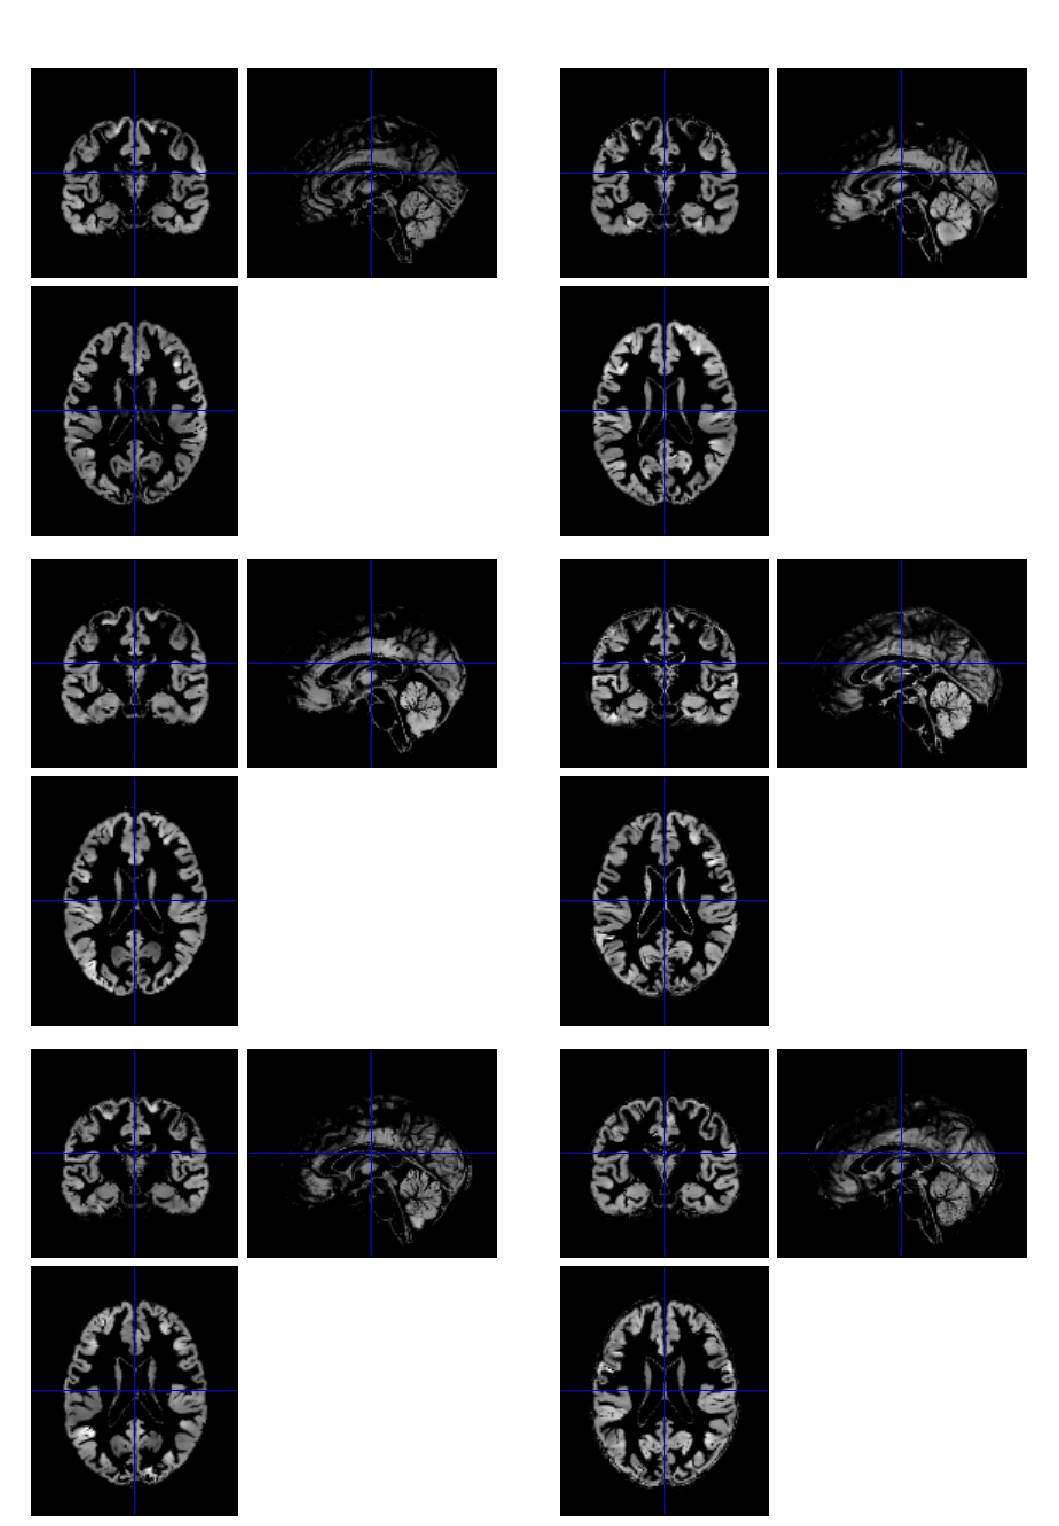
\includegraphics[width=1\textwidth]{mwc1_ixi}
\end{columns}
\end{frame}



\begin{frame}
\frametitle{``Scalar Momentum'' Features}
\begin{columns}[c]
\column{0.33\textwidth}
``Scalar momentum'' actually has two components because GM was matched with GM and WM was matched with WM.
\column{0.33\textwidth}
First Momentum Component

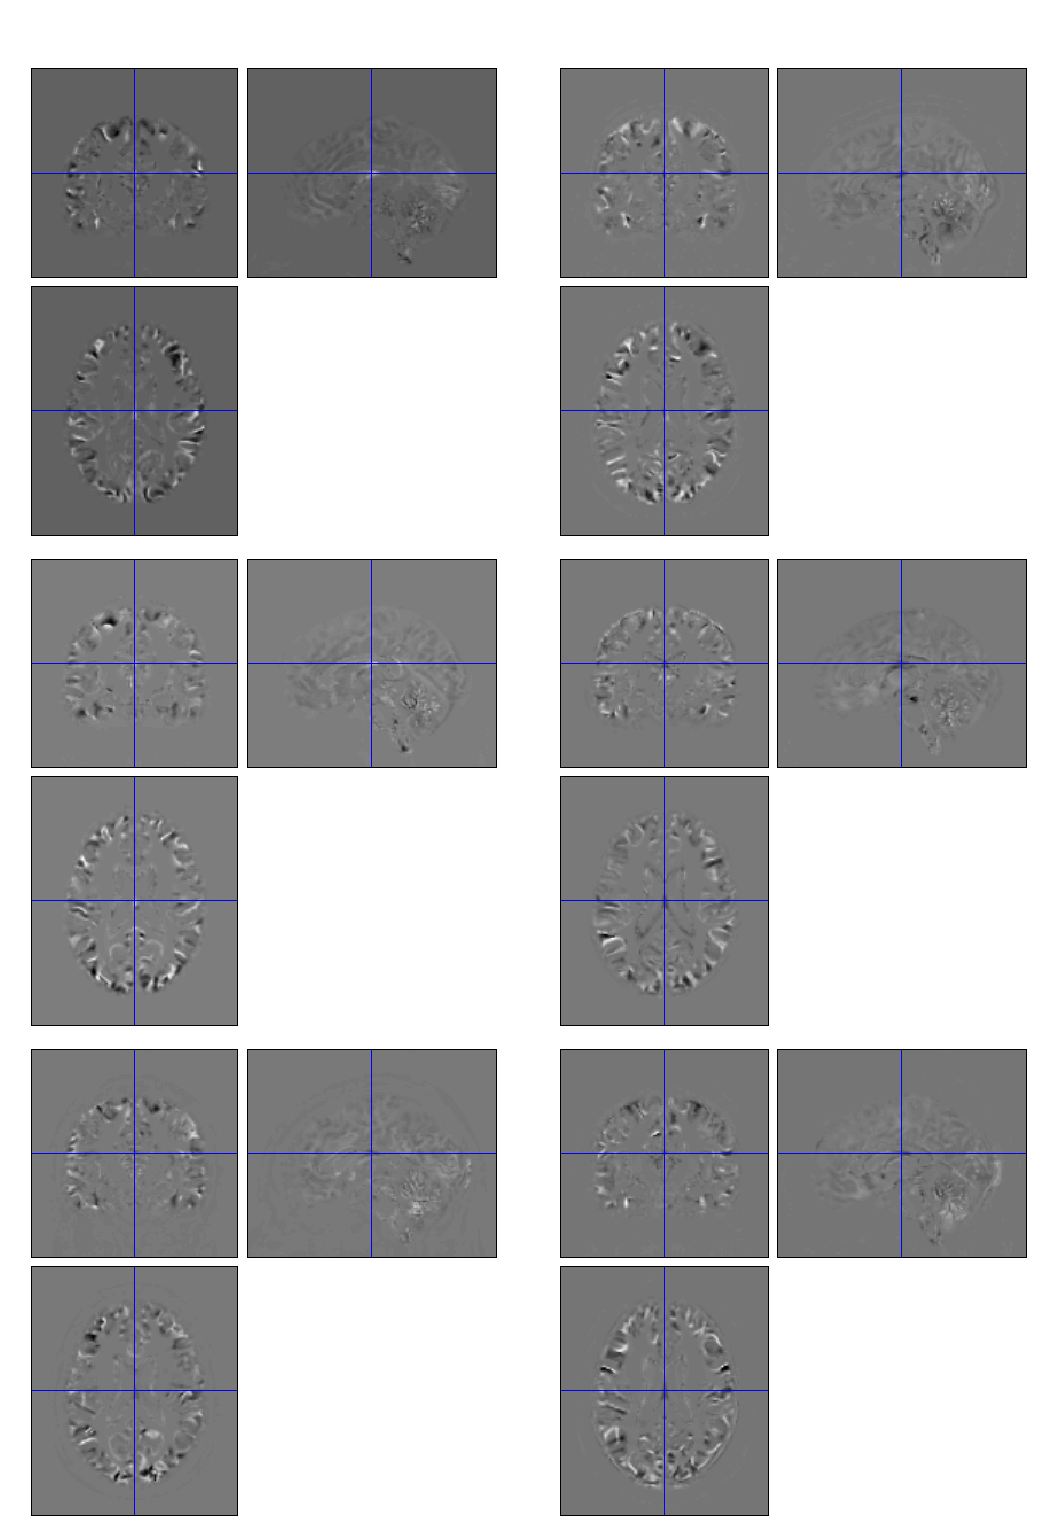
\includegraphics[width=1\textwidth]{resids1_ixi}
\column{0.33\textwidth}
Second Momentum Component

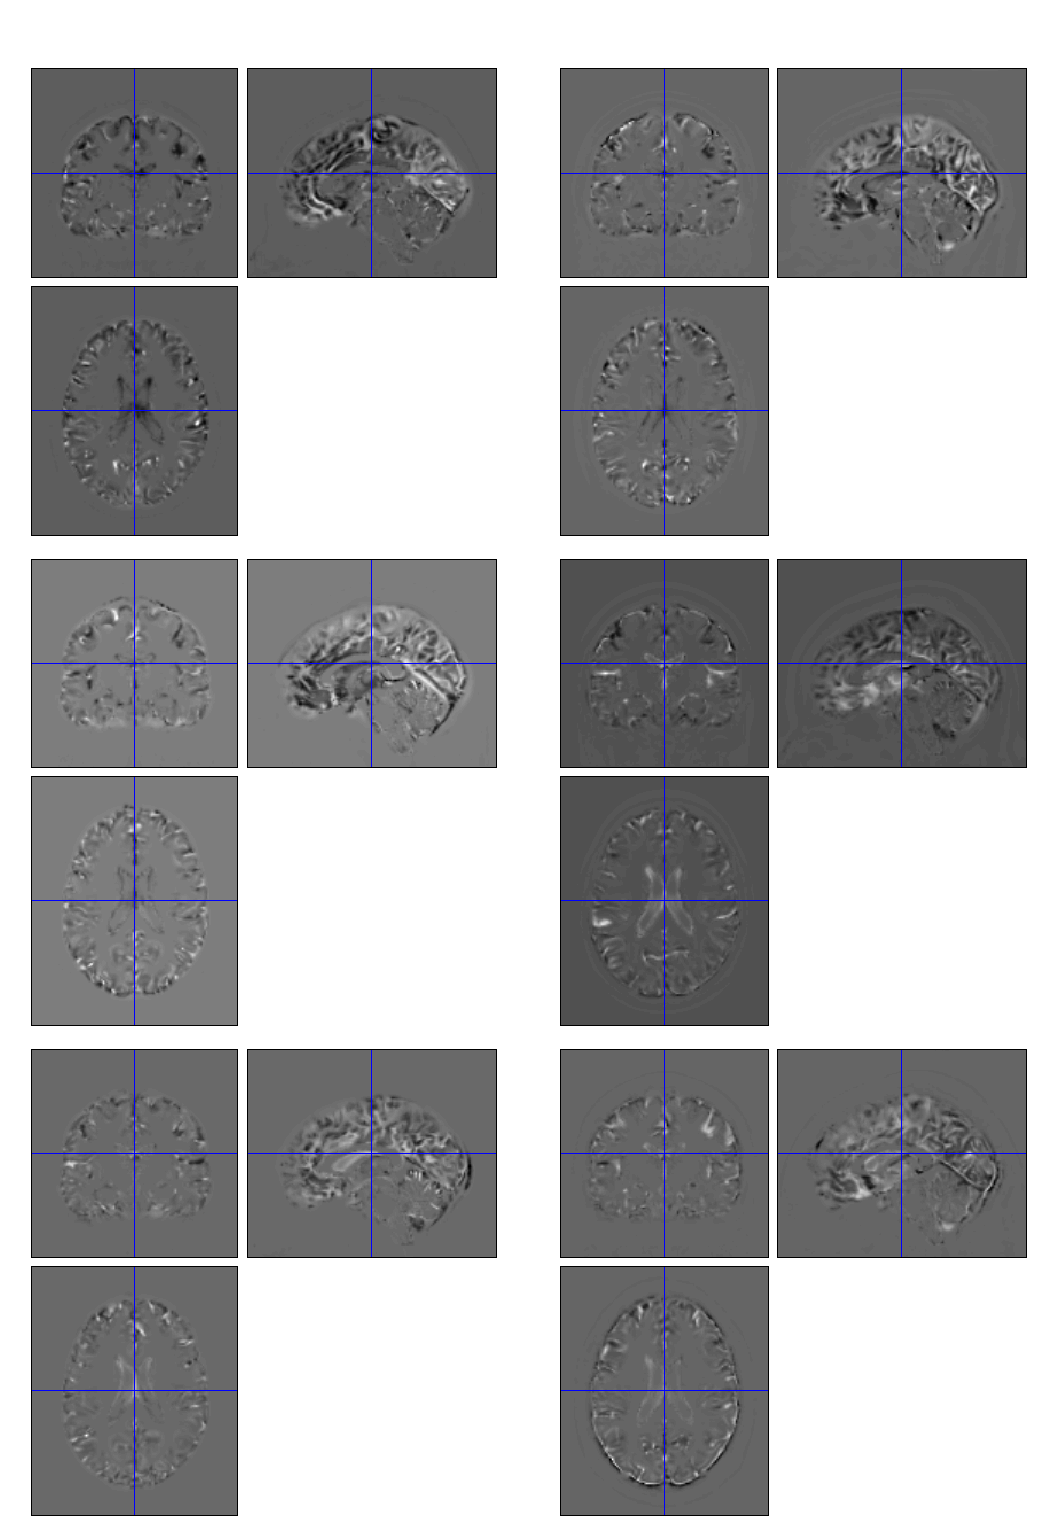
\includegraphics[width=1\textwidth]{resids2_ixi}
\end{columns}
\end{frame}



\begin{frame}
\frametitle{Age Regression}
Linear Gaussian Process Regression to predict subject ages.
\begin{columns}[c]
\column{0.5\textwidth}
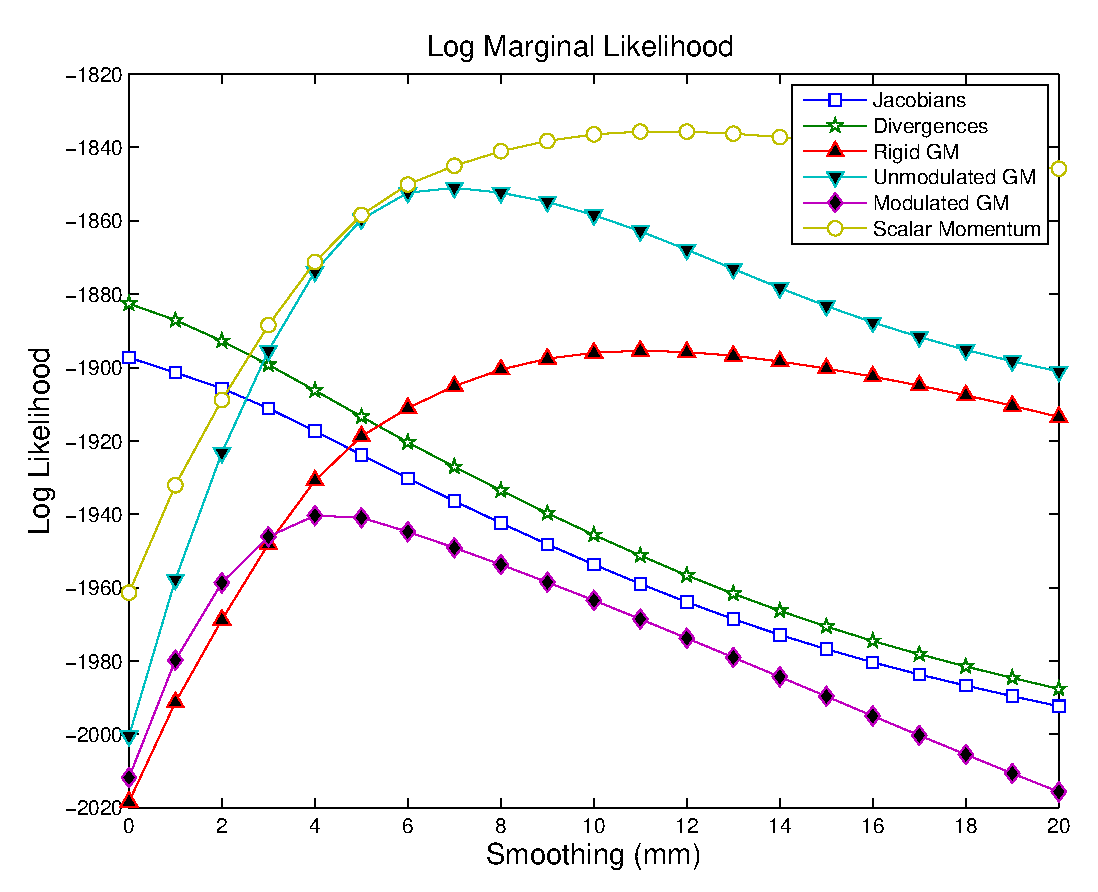
\includegraphics[width=1\textwidth]{age_loglikelihood}
\column{0.5\textwidth}
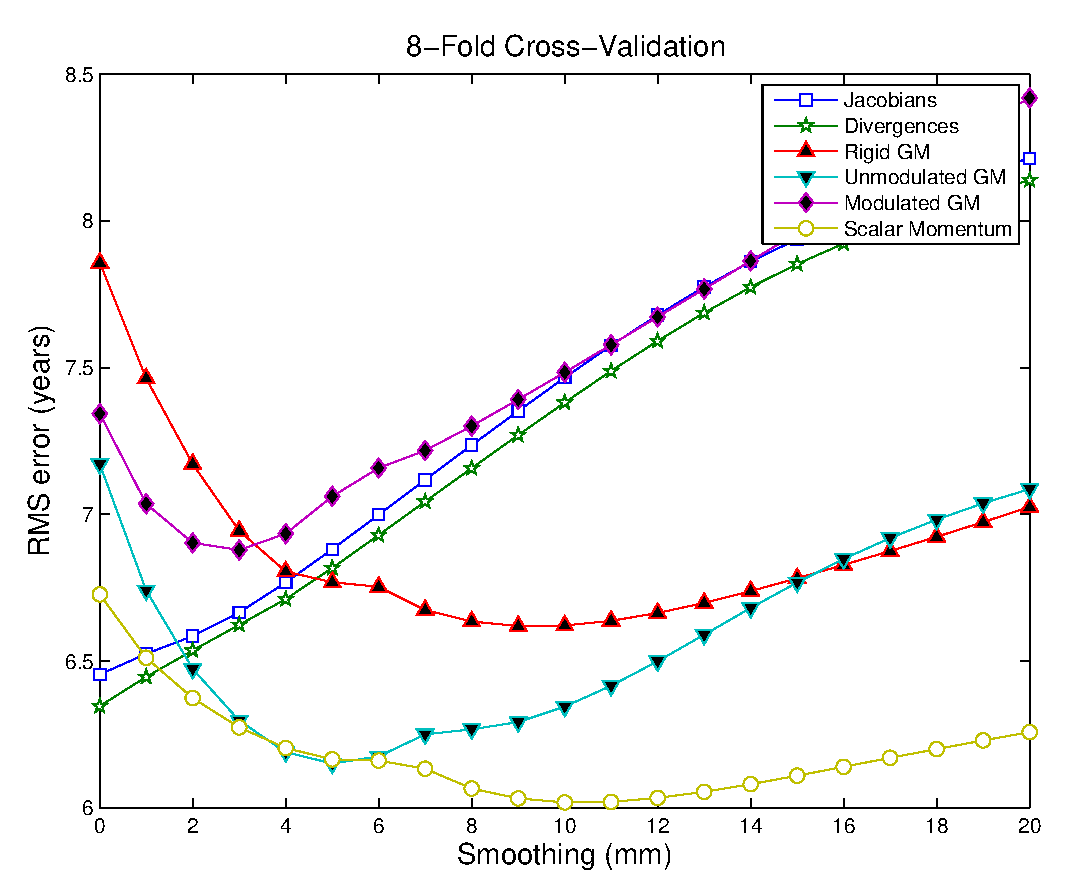
\includegraphics[width=1\textwidth]{age_rms}
\end{columns}

\begin{tiny}
Rasmussen, CE \& Williams, CKI. \emph{Gaussian processes for machine learning}. Springer (2006).

\end{tiny}
\end{frame}

%%%%%%%%%%%%%%%%%%%%%%%%%%%%%%%%%%%%%%%%%%%%%%%%%%%%%%%%%%%%%%%
\begin{frame}
\frametitle{Sex Classification}
Linear Gaussian Process Classification (EP) to predict sexes.
\begin{columns}[c]
\column{0.5\textwidth}
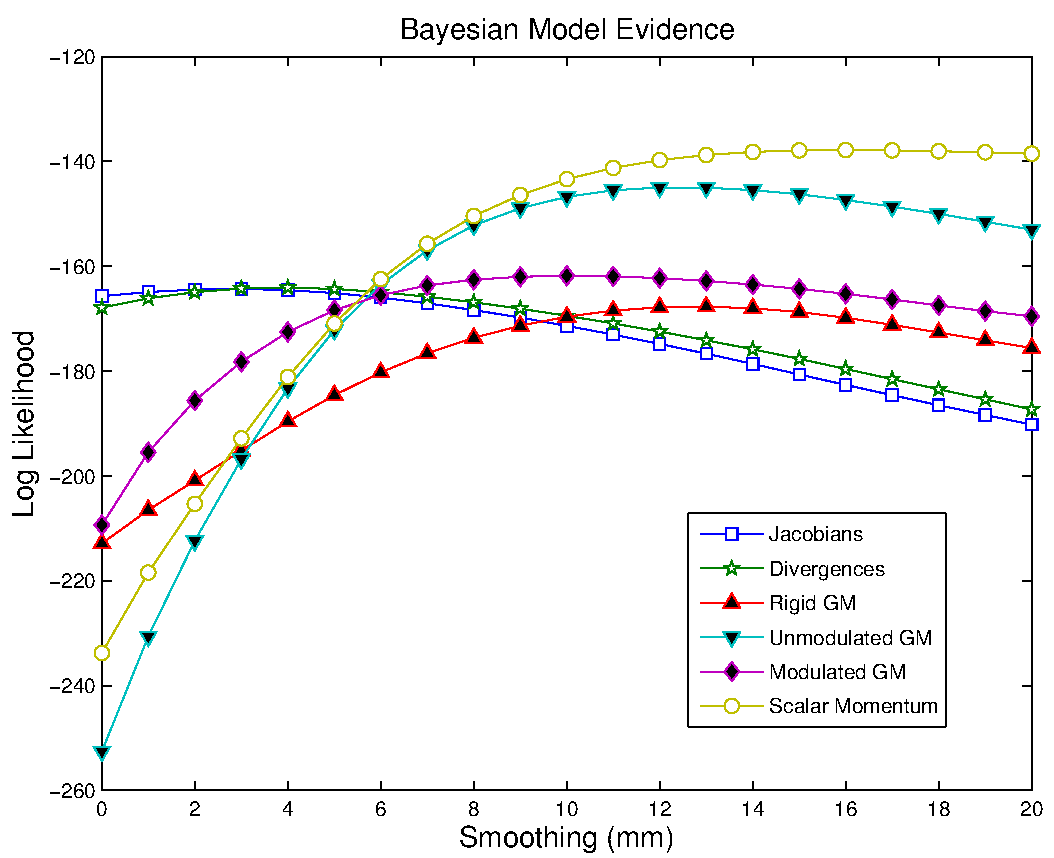
\includegraphics[width=1\textwidth]{sex_loglikelihood}
\column{0.5\textwidth}
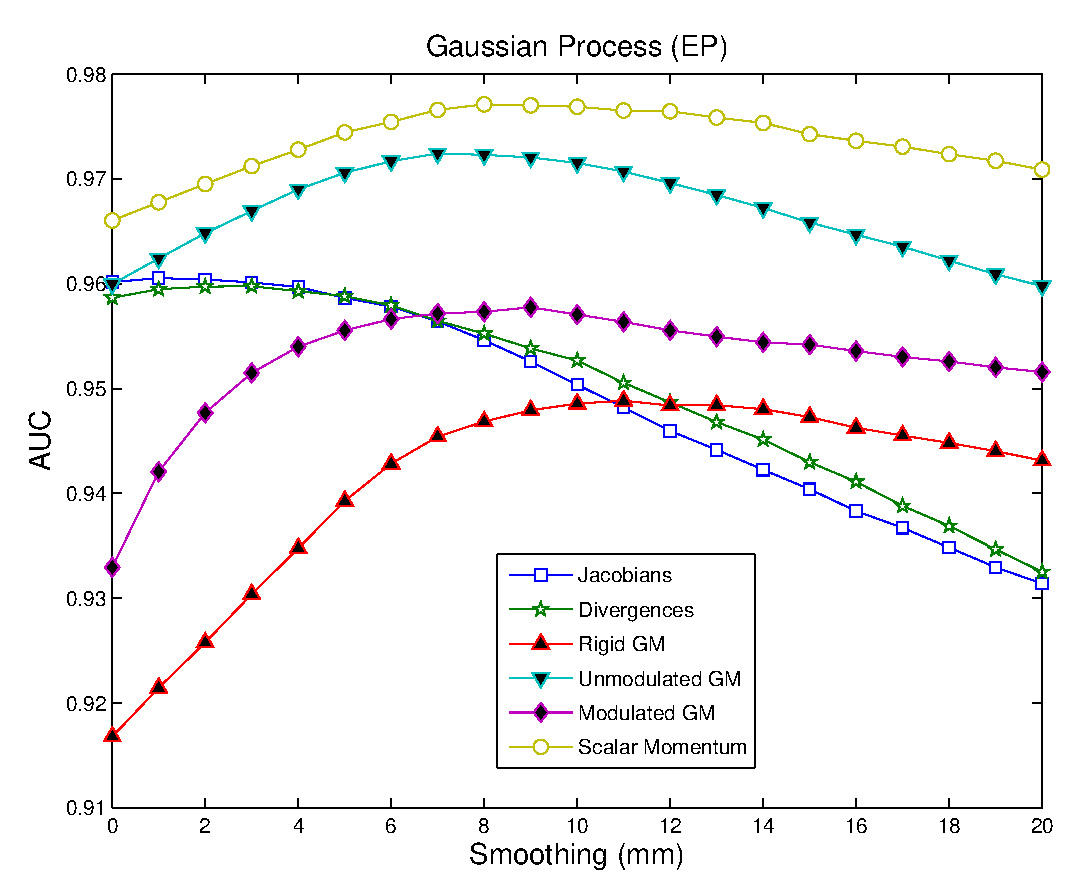
\includegraphics[width=1\textwidth]{sex_auc_GP}
\end{columns}

\begin{tiny}
Rasmussen, CE \& Williams, CKI. \emph{Gaussian processes for machine learning}. Springer (2006).

\end{tiny}
\end{frame}

%%%%%%%%%%%%%%%%%%%%%%%%%%%%%%%%%%%%%%%%%%%%%%%%%%%%%%%%%%%%%%%
%\begin{frame}
%\frametitle{Sex Classification}
%Linear SVM versus Gaussian Process Classification (EP).
%\begin{columns}[c]
%\column{0.5\textwidth}
%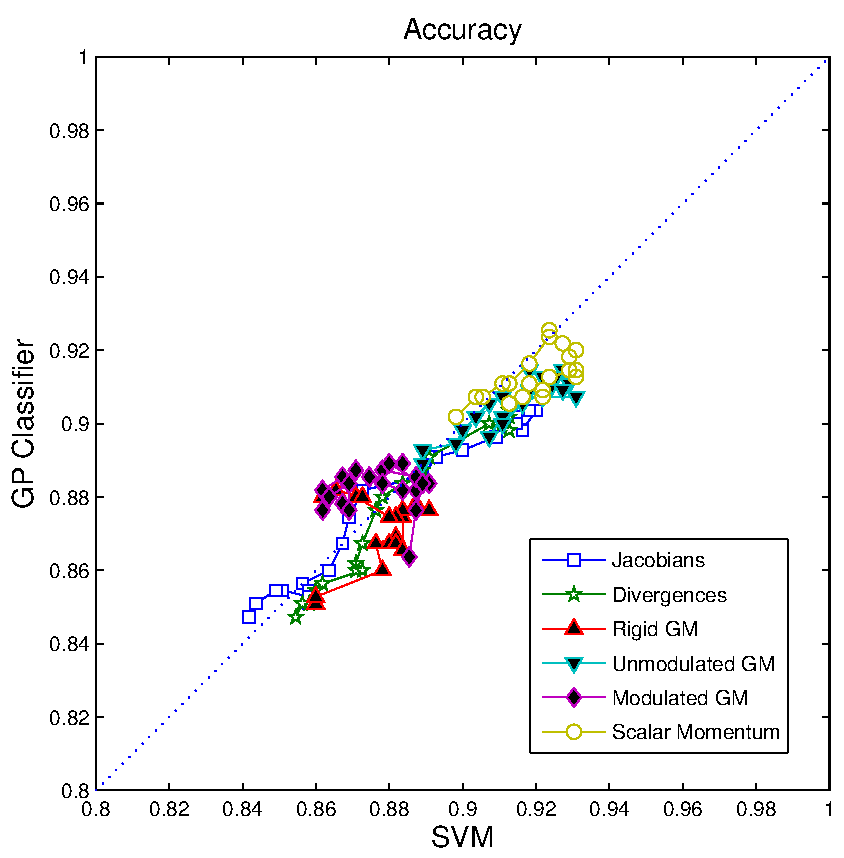
\includegraphics[width=1\textwidth]{sex_SVM_v_GP_acc}
%\column{0.5\textwidth}
%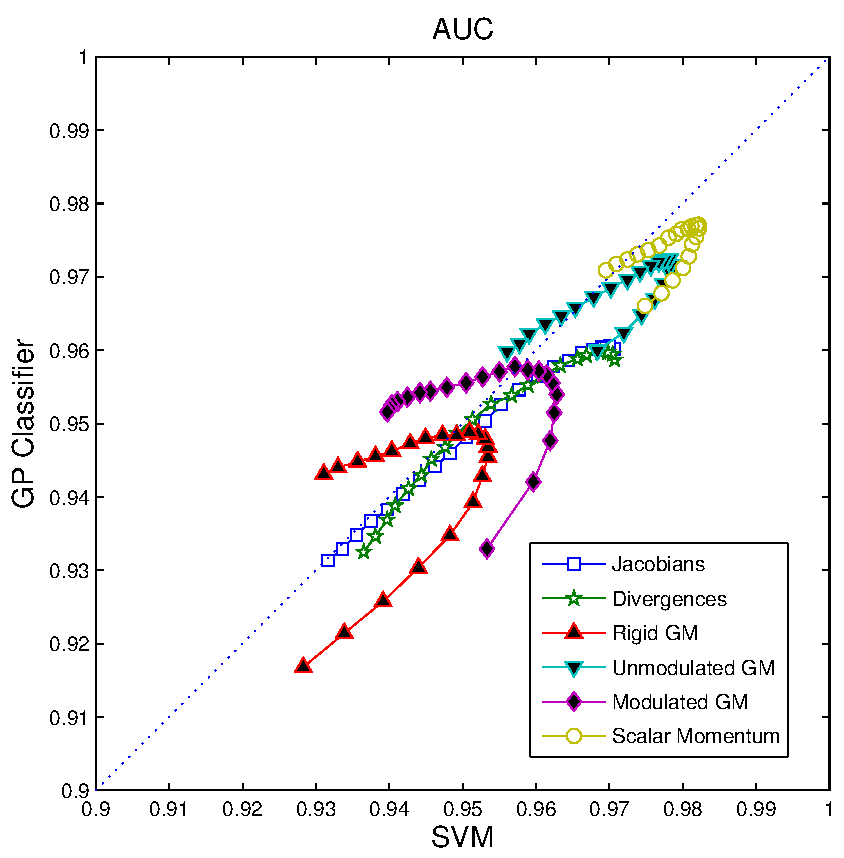
\includegraphics[width=1\textwidth]{sex_SVM_v_GP_AUC}
%\end{columns}
%\end{frame}

%%%%%%%%%%%%%%%%%%%%%%%%%%%%%%%%%%%%%%%%%%%%%%%%%%%%%%%%%%%%%%%


\begin{frame}
\frametitle{Predictive Accuracies}
\begin{columns}[c]
\column{0.5\textwidth}

Age

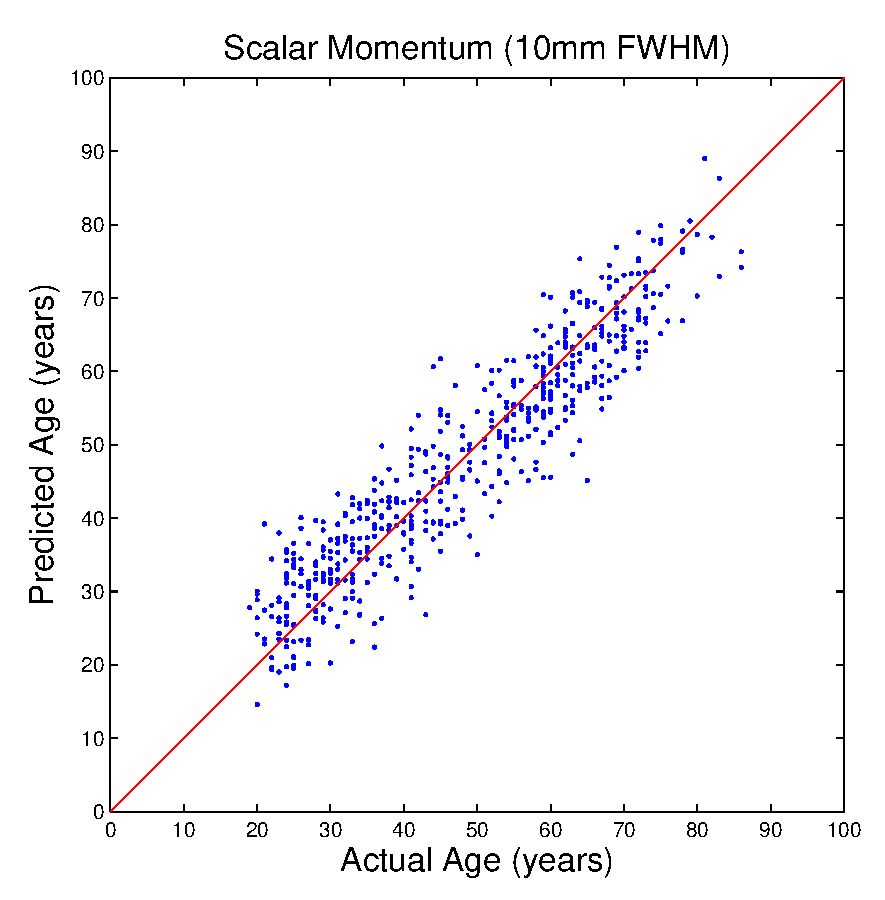
\includegraphics[width=1\textwidth]{age_predictions}
\column{0.5\textwidth}

Sex

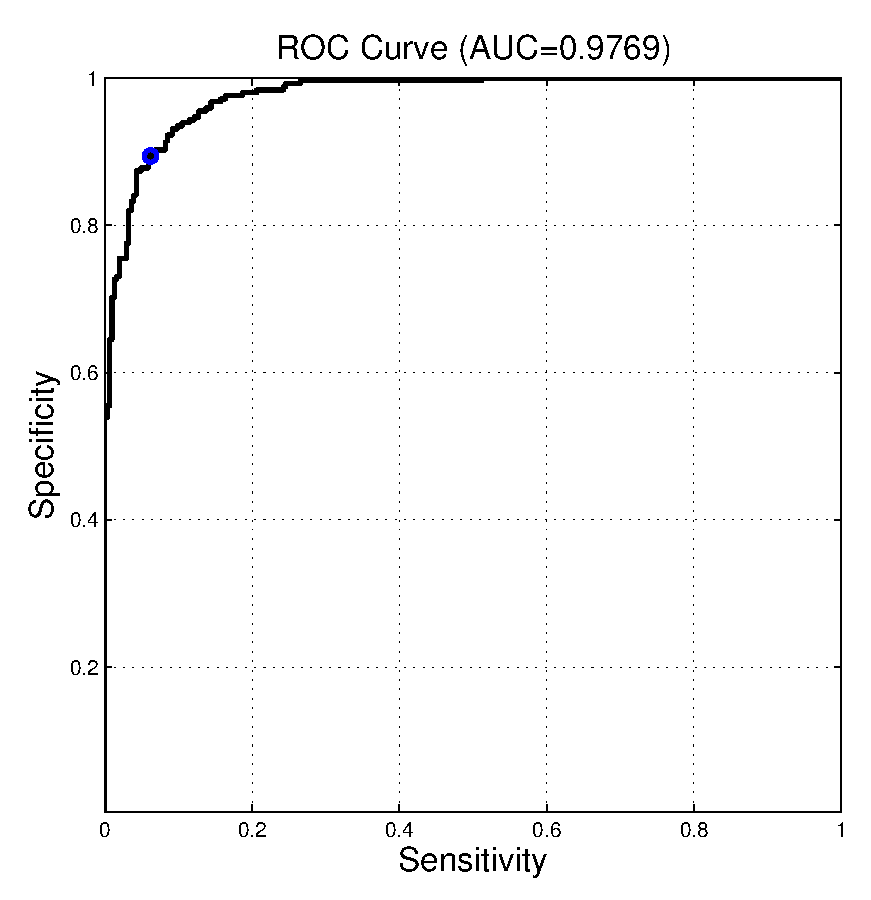
\includegraphics[width=1\textwidth]{sex_roc}
\end{columns}
\end{frame}

\begin{frame}
\frametitle{Conclusions}
\begin{itemize}
\item{Scalar momentum (with about 10mm smoothing) appears to be a useful feature set.}
\item{Jacobian-scaled warped GM is surprisingly poor.}
%\item{SVC slightly more accurate than GP (but we knew that already).}
\item{Amount of spatial smoothing makes a big difference.}
\item{Further dependencies on the details of the registration still need exploring.}
\end{itemize}
\end{frame}
%%%%%%%%%%%%%%%%%%%%%%%%%%%%%%%%%%%%%%%%%%%%%%%%%%%%%%%%%%%%%%%
%\begin{frame}
%\frametitle{Additional references}
%\begin{itemize}
%\item{Ashburner, J \& Kl\"oppel, K. \emph{Multivariate models of inter-subject anatomical variability}. NeuroImage 56(2):422--439 (2011).}
%\item{Ashburner, J \& Friston, KJ. \emph{Diffeomorphic registration using geodesic shooting and Gauss-Newton optimisation}. NeuroImage 55(3):954--967 (2011).}
%\end{itemize}
%\end{frame}

